\documentclass[sigconf]{acmart}

\usepackage{booktabs} % For formal tables

\usepackage{amsmath}
\usepackage{float}
\usepackage{hyperref}
\usepackage{listings}
\usepackage{algorithm}
\usepackage[noend]{algpseudocode}
\usepackage{graphicx}
\usepackage{courier}
\usepackage{float}
\usepackage{color}
\usepackage[margin=10pt,font=small,labelfont=bf,
  labelsep=endash]{caption}
\usepackage{ulem}

\usepackage{syntax} % for writing BNF grammar

\usepackage{forest}
\usepackage{framed}

\usepackage{tikz}
\usetikzlibrary{matrix}
\usetikzlibrary{shapes.multipart}
\usetikzlibrary{patterns}
\usetikzlibrary{positioning,fit,calc}
\usetikzlibrary{decorations.pathmorphing}
\usetikzlibrary{decorations.pathreplacing}
\usetikzlibrary{quotes}
\usetikzlibrary{graphs}
\usetikzlibrary{arrows.meta}
\usetikzlibrary{shapes}
% \usetikzlibrary{graphs,graphdrawing}
% \usegdlibrary{layered}
% \usetikzlibrary{graphdrawing,graphs,calc}
% \usegdlibrary{layered}

\usepackage{smartdiagram}

% \usetikzlibrary{external}
% \tikzexternalize % activate!
% \tikzset{external/force remake}

%% To generate figure, uncomment above three lines, and execute:
%% pdflatex -shell-escape helium.tex

\usepackage{csvsimple}
\usepackage{multirow}


\lstset{basicstyle=\footnotesize\ttfamily,breaklines=true}
% \lstset{frame=b}
\lstset{float,floatplacement=H,captionpos=b}
% \lstset{numbers=left}
\lstset{language=C}
\lstset{showstringspaces=false}
\lstset{breakindent=10pt}
% \lstset{framextopmargin=10pt}
% \lstset{framextopmargin=50pt,frame=t}
% \lstset{float=htb,language=C,frame=single, basicstyle=\small, stringstyle=\ttfamily}
% \lstset{escapeinside={(*@}{@*)}}
% \usepackage{xcolor}
\lstdefinestyle{base}{
  language=C,
  emptylines=1,
  breaklines=true,
  aboveskip=0em,
  belowskip=0em,
  % float,
  % floatplacement=H,
  basicstyle=\footnotesize\ttfamily\color{black},
  moredelim=**[is][\color{blue}]{@}{@},
  moredelim=**[is][\color{purple}]{~1}{~1},
  moredelim=**[is][\color{brown}]{~2}{~2},
  moredelim=**[is][\color{gray}]{~3}{~3},
  moredelim=**[is][\color{orange}]{~4}{~4},
  moredelim=**[is][\color{violet}]{~5}{~5},
}
\lstdefinestyle{graycode} {
  language=C,
  emptylines=1,
  breaklines=true,
  basicstyle=\footnotesize\ttfamily\color{gray!50},
  moredelim=**[is][\color{blue}]{@}{@},
}
\lstset{style=base}


\title{How to compute}
% \lstset{numbers=left}
\begin{document}

\begin{figure*}
  \centering
  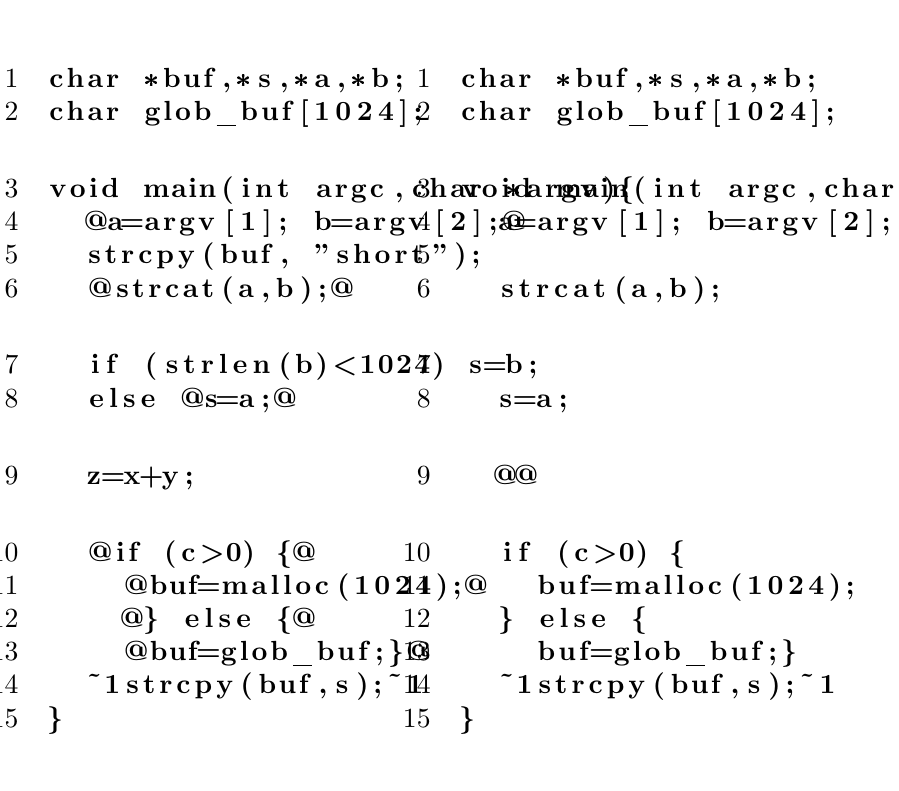
\begin{tikzpicture}[every label quotes/.style={left, font=\footnotesize},
      cfg/.style={draw,rectangle,rounded corners},
      tf/.style={text=\scriptsize},
      trans/.style={align=center,draw,rounded corners,rectangle
        split,rectangle split parts=2,draw,dashed,fill=gray!10!white,minimum width=5cm,font=\scriptsize\bfseries},
      bench/.style={draw,fill=gray!20!white},
      slice/.style={draw,ultra thick},
      merge label/.style={red,font=\scriptsize\bfseries,draw,rotate=-45,label position=40},
      every label/.style={font=\normalsize},
      num/.style={draw,circle},
      label position={0},
      font=\bfseries,
      ]

    \matrix (full) [
      matrix anchor=north east,
      every node/.style={
        % draw,
        inner ysep=0,
        text width=5cm,
        % inner xsep=10pt,
      },
      % column sep=3pt,
      anchor=north west,
      every label quotes/.style={below,font=\footnotesize},
      % align=center,
      % column sep=10pt,
      % draw
      ] {
      \node {
\begin{lstlisting}[numbers=left, firstnumber=1]
char *buf,*s,*a,*b;
char glob_buf[1024];
\end{lstlisting}
      };&
      \node {
\begin{lstlisting}[numbers=left, firstnumber=1]
char *buf,*s,*a,*b;
char glob_buf[1024];
\end{lstlisting}
      };\\
      \node {
\begin{lstlisting}[numbers=left, firstnumber=3]
void main(int argc,char *argv){
  @a=argv[1]; b=argv[2];@
  strcpy(buf, "short");
  @strcat(a,b);@
\end{lstlisting}
      };&
      \node {
\begin{lstlisting}[numbers=left, firstnumber=3]
void main(int argc,char *argv){
  a=argv[1]; b=argv[2];

  strcat(a,b);
\end{lstlisting}
      };\\
      \node {
\begin{lstlisting}[numbers=left, firstnumber=7]
  if (strlen(b)<1024) s=b;
  else @s=a;@
\end{lstlisting}
      };&
      \node {
\begin{lstlisting}[numbers=left, firstnumber=7]

  s=a;
\end{lstlisting}
      };\\
      \node {
\begin{lstlisting}[numbers=left, firstnumber=9]
  z=x+y;
\end{lstlisting}
      };&
      \node {
\begin{lstlisting}[numbers=left, firstnumber=9]
  @@
\end{lstlisting}
      };\\
      \node {
\begin{lstlisting}[numbers=left, firstnumber=10]
  @if (c>0) {@
    @buf=malloc(1024);@
    @} else {@
    @buf=glob_buf;}@
  ~1strcpy(buf,s);~1
}
\end{lstlisting}
      };&
      \node {
\begin{lstlisting}[numbers=left, firstnumber=10]
  if (c>0) {
    buf=malloc(1024);
  } else {
    buf=glob_buf;}
  ~1strcpy(buf,s);~1
}
\end{lstlisting}
      };\\
      % \node [align=left] {
      %   \quad \quad Original Program
      % };&
      % \node [align=left] {
      %   \quad \quad Bug Signature
      % };\\
    };
  \end{tikzpicture}
  \caption{Original \& Bug Signature Program}
\end{figure*}

\end{document}
